% =====================================================================
%  Основное содержимое отчёта (часть 1): структура, технологии,
%  алгоритмы, интерфейс.
% =====================================================================

\labpart{Структура разработанной системы}

Синтез речи реализован как новый сценарий использования поверх
архитектуры ЛР1--ЛР4 (см. \texttt{docs/ARCHITECTURE.md}): границы
сервисов по-прежнему проведены по зоне ответственности, а не по
лабораторной работе. Синтез речи тянет за собой тяжёлую зависимость
(среда исполнения нейросетей \texttt{onnxruntime}) и отдельно
скачиваемые файлы голосов, поэтому, по тому же принципу изоляции
тяжёлых ML-зависимостей, что и \texttt{lang-id-service} (ЛР2) и
\texttt{mt-service} (ЛР4), он выделен в новый микросервис
\texttt{speech-service}. Базе данных для синтеза речи ничего хранить не
нужно, поэтому схема БД в этой лабораторной работе не менялась.
Структура системы на уровне контейнеров (C4, уровень 2) показана на
рисунке~\ref{fig:architecture-c4}; компоненты и связи, добавленные в
этой лабораторной работе, выделены зелёным цветом.

\pumldiagram{architecture-c4}{Диаграмма контейнеров разработанной системы (нотация C4); зелёным -- новое в ЛР8}{architecture-c4}{0.95}

Ответственность компонентов распределена следующим образом.
\begin{itemize}
  \item \textbf{\texttt{speech-service}} (Python, FastAPI, Piper) --
  единственный компонент, который знает, как получить звук из текста.
  Эндпоинт \texttt{POST /tts} принимает текст (от 1 до 5000 символов),
  идентификатор голоса и темп и \emph{потоком} возвращает WAV: сервис
  отдаёт заголовок и звук первого предложения, не дожидаясь синтеза
  всего текста. Голоса скачиваются на этапе сборки образа и
  загружаются в память лениво -- при первом обращении к голосу.
  Контейнер ограничен по ресурсам (4~ГиБ памяти, 4 ядра CPU), чтобы
  чрезмерно большой запрос не мог исчерпать ресурсы хоста и остановить
  остальные сервисы;
  \item \textbf{\texttt{api}} (Python, FastAPI) -- шлюз для интерфейса:
  эндпоинт \texttt{POST /speech/tts} проверяет запрос (тот же лимит в
  5000 символов, чтобы не гонять по сети заведомо неверный запрос) и
  проксирует поток из \texttt{speech-service} без буферизации. Слой
  \texttt{application/speech} (\texttt{SpeechSynthesisService}) не
  зависит от HTTP-деталей: клиент \texttt{speech-service}
  (\texttt{SpeechServiceClient}) передаётся ему как зависимость, поэтому
  в тестах подменяется заглушкой;
  \item \textbf{\texttt{frontend}} (React, TypeScript) -- хранит настройки
  голоса, режет текст на фрагменты, запрашивает у \texttt{api} звук
  каждого фрагмента и проигрывает его через Web Audio API. Состоит из
  трёх контекстов и трёх компонентов, перечисленных в
  таблице~\ref{tab:frontend-components}.
\end{itemize}

\begin{table}[H]
  \centering
  \caption{Компоненты интерфейса, реализующие синтез речи}
  \label{tab:frontend-components}
  \small
  \begin{tabular}{|p{0.36\textwidth}|p{0.55\textwidth}|}
    \hline
    \textbf{Компонент} & \textbf{Назначение} \\
    \hline
    \texttt{SpeechSettingsContext} & Настройки голоса, темпа, громкости; сохраняются в \texttt{localStorage} браузера и переживают перезагрузку страницы \\
    \hline
    \texttt{SpeechPlaybackContext} & Очередь фрагментов: запрос звука, декодирование, воспроизведение, предвыборка следующего фрагмента, остановка \\
    \hline
    \texttt{speechChunking.ts} & Разбиение текста на фрагменты для озвучивания \\
    \hline
    \texttt{SpeakButton} & Кнопка «Озвучить / Остановить» рядом с любым текстом: документом, рефератом, переводом; подсвечивается звуковой волной, пока звучит её текст \\
    \hline
    \texttt{ClipboardSpeakButton} & Кнопка «Озвучить из буфера»: читает текст из буфера обмена и озвучивает его \\
    \hline
    Вкладка «Синтез речи» страницы «Настройки» & Выбор голоса, ползунки темпа и громкости, поле произвольного текста для проверки \\
    \hline
  \end{tabular}
\end{table}

\labpart{Технологии и методики}

\textbf{Выбор технологии синтеза.} Методичка предлагает FreeTTS,
Microsoft Speech API, Google Speech API, Web Speech API и нейросетевые
библиотеки. Все варианты, кроме последнего, имеют существенные
ограничения для этой системы: Microsoft Speech API привязан к
Windows, тогда как система развёртывается одной командой в Docker и
не должна зависеть от операционной системы хоста; облачные API
требуют ключей, доступа в интернет и передачи текста документов
третьей стороне; Web Speech API отдаёт то голоса, что установлены в
конкретной операционной системе и браузере, поэтому результат
невозможно воспроизвести на другой машине, и набор голосов не
контролируется системой; FreeTTS даёт заметно более механическое
звучание. Поэтому выбрана нейросетевая система \textbf{Piper}
(\texttt{piper-tts} 1.8.0): голоса представляют собой модели VITS
(вариационный автокодировщик с состязательным обучением), экспортированные в
формат ONNX, качества \emph{medium} (частота дискретизации 22\,050~Гц,
моно, 16 бит). Синтез идёт на CPU быстрее реального времени (см.
раздел «Результаты тестирования»), работает без интернета, а набор
голосов задан образом контейнера и потому одинаков на любой машине.

\textbf{Голоса.} Для варианта~1 (английский язык) доступно 10 голосов
одного качества (\emph{medium}): 7 американских
(Amy, Lessac, HFC Female, Kristin -- женские; Ryan, HFC Male, Joe --
мужские) и 3 британских (Alba и Jenny -- женские, Alan -- мужской).
Голос по умолчанию -- \texttt{en\_US-amy-medium}.

\textbf{Темп.} В Piper скорость речи задаётся параметром
\texttt{length\_scale} -- множителем длительности фонем. Пользователь
выбирает темп $r$ от $0{,}5\times$ до $2{,}0\times$ с шагом $0{,}1$;
в \texttt{length\_scale} он переводится обратным значением:
\begin{equation}
  \texttt{length\_scale} = \frac{1}{r},
\end{equation}
поэтому темп $2\times$ сокращает звучание вдвое, а $0{,}5\times$ --
удваивает его, не меняя высоты голоса (в отличие от простого
ускорения воспроизведения готовой записи). Точность этого соотношения
проверена измерением (табл.~\ref{tab:tempo}).

\textbf{Громкость.} Громкость регулируется на стороне браузера узлом
\texttt{GainNode} Web Audio API (коэффициент от 0 до 1): она не требует
повторного синтеза, поэтому изменение громкости не влияет на нагрузку
на сервер.

\textbf{Потоковый WAV.} Piper выдаёт звук по предложениям, а общий
размер звука до окончания синтеза неизвестен. Поэтому
\texttt{speech-service} отправляет WAV-заголовок с размером-заглушкой
\texttt{0xFFFFFFFF} (принятая практика для потокового WAV), а затем
блоки PCM по мере готовности. Браузеры не всегда корректно
декодируют такой заголовок, поэтому интерфейс, получив ответ, заменяет
поля размера в заголовке на реальные значения.

\textbf{Воспроизведение через Web Audio API, а не через элемент
\texttt{audio}.} Chrome разрешает воспроизведение звука только в
ответ на действие пользователя (нажатие); при озвучивании по
фрагментам следующий фрагмент запускается уже не в обработчике нажатия,
а после завершения предыдущего, и элемент \texttt{audio} в этот
момент мог бы быть заблокирован. Контекст \texttt{AudioContext}
достаточно один раз «разбудить» по нажатию, после чего все
последующие фрагменты играют без ограничений.

\labpart{Основные алгоритмы}

\textbf{Общая схема обмена.} Последовательность обмена сообщениями при
синтезе одного фрагмента текста показана на
рисунке~\ref{fig:tts-sequence}. Ключевое свойство схемы -- потоковость
на всём пути: звук первого предложения возвращается интерфейсу,
пока сервис ещё синтезирует следующие.

\pumldiagram{tts-sequence}{Обмен сообщениями при синтезе речи}{tts-sequence}{0.95}

\textbf{Разбиение текста на фрагменты.} Научная статья -- это
несколько тысяч символов, а синтез всего текста одним запросом
заставил бы пользователя ждать, пока будет готов звук всей статьи
(измерено в разделе «Результаты тестирования»). Поэтому текст режется на
фрагменты, и озвучивание начинается сразу после синтеза
первого. Алгоритм (рисунок~\ref{fig:chunking}) собирает
фрагменты из целых предложений: предложения по очереди добавляются в
текущий фрагмент, пока его длина не превысит целевую (120 символов);
предложение длиннее максимума (240 символов) режется жёстко.
Границы фрагментов совпадают с границами предложений, поэтому
интонация не ломается посреди фразы, а максимальная длина фрагмента
остаётся намного ниже серверного лимита в 5000 символов.

\pumldiagram{chunking}{Разбиение текста на фрагменты для озвучивания}{chunking}{0.85}

\textbf{Воспроизведение с упреждающей выборкой.} Пока звучит
фрагмент~$i$, запрос на синтез фрагмента~$i+1$ уже отправлен
(рисунок~\ref{fig:tts-playback}). Если синтез быстрее звучания, а это
так, пока синтез идёт быстрее реального времени, то пауз между
фрагментами нет вообще: к моменту окончания фрагмента~$i$ звук
фрагмента~$i+1$ уже готов. Остановка пользователем прерывает все
незавершённые запросы через \texttt{AbortController}, чтобы сервер не
тратил ресурсы на синтез уже ненужного текста.

\pumldiagram{tts-playback}{Воспроизведение фрагментов с упреждающей выборкой}{tts-playback}{0.42}

\labpart{Способы ввода текста и пользовательский интерфейс}

Методичка допускает три способа получить текст для озвучивания:
ввод, копирование через буфер обмена либо указатель мыши в другом
приложении. Реализованы первые два:
\begin{itemize}
  \item \textbf{Ввод.} Произвольный текст вводится в поле на вкладке
  «Синтез речи» страницы «Настройки». Кроме того, кнопка «Озвучить»
  расположена рядом с каждым текстом, с которым работает система:
  документом коллекции (диалог просмотра/редактирования документа --
  текст научной статьи из предметной области варианта), рефератом
  (ЛР3, вкладки алгоритмического, TextRank- и эмбеддинг-методов) и
  результатом машинного перевода (ЛР4);
  \item \textbf{Буфер обмена.} Кнопка «Озвучить из буфера» читает
  текст через \texttt{navigator.clipboard.readText()} и озвучивает
  его, одновременно подставляя в поле проверки, чтобы пользователь
  видел, что именно читается. Так можно озвучить текст из любого
  другого приложения или страницы: выделить, скопировать (Ctrl+C) и
  нажать кнопку. Если браузер не разрешает доступ к буферу, а также
  если буфер пуст, интерфейс сообщает об этом;
  \item \textbf{Указатель мыши в другом приложении} не реализован:
  веб-страница не может получить выделенный текст из чужого окна --
  это ограничение безопасности браузера, а не системы. Его роль
  выполняет буфер обмена, разрешённый заданием как равноправная
  альтернатива.
\end{itemize}

Параметры чтения меняются на той же вкладке: голос (список из 10
голосов), темп (ползунок $0{,}5$--$2{,}0\times$) и громкость (ползунок
0--100\,\%). Настройки применяются к следующему озвучиванию сразу, без
перезагрузки; до нажатия на кнопку «Озвучить» их можно проверить на
примере текста в том же поле. Помимо кнопок, озвучиванием можно
управлять голосом (команды «read this» и «stop reading», см. ЛР9).


\begin{figure}[H]
  \centering
  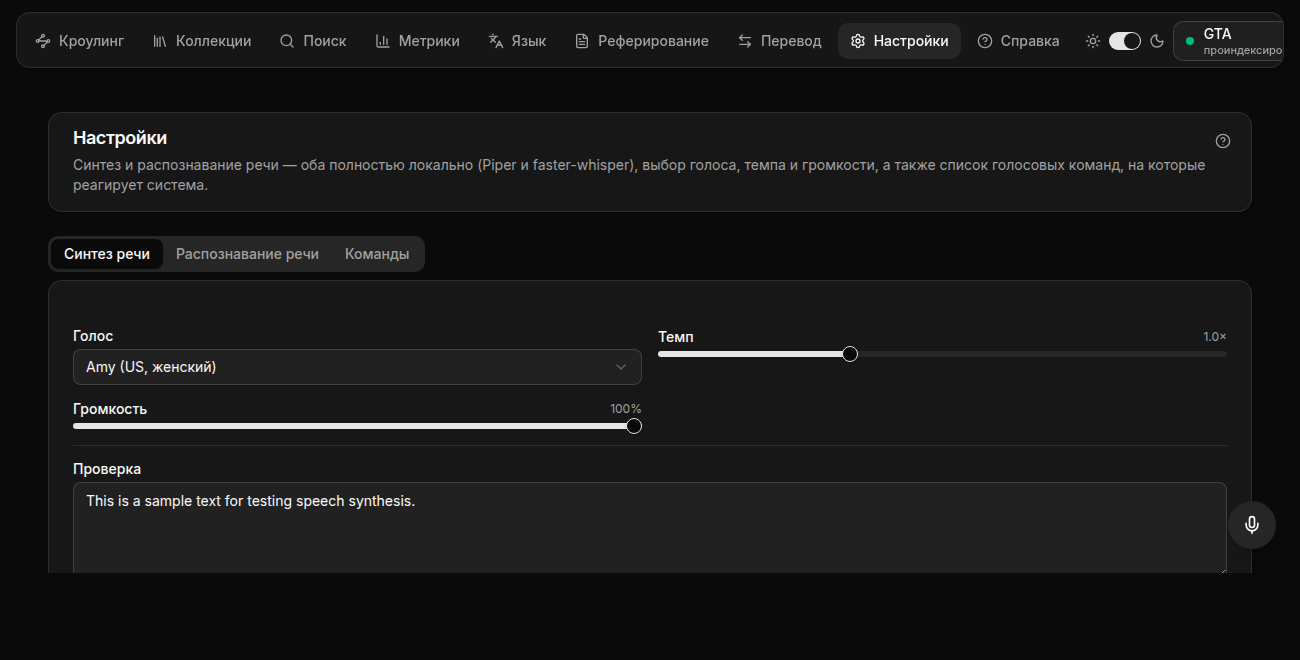
\includegraphics[width=\textwidth]{lab/pictures/settings_tts.png}
  \caption{Вкладка «Синтез речи» страницы «Настройки»: голос, темп, громкость, поле текста, кнопки «Озвучить из буфера» и «Озвучить»}
  \label{fig:settings-tts}
\end{figure}


\labpartbreak{Результаты тестирования}

Тестирование проводилось на работающей системе (\texttt{docker compose}),
через тот же эндпоинт \texttt{POST /speech/tts}, которым пользуется
интерфейс; контейнер \texttt{speech-service} был ограничен четырьмя
ядрами CPU и 4~ГиБ памяти (см. «Структура разработанной системы»).
Тексты -- предложения из области варианта (научные статьи по computer
science). Каждое измерение повторялось трижды после «прогрева» голоса,
в таблицах приведены средние значения. Под \emph{коэффициентом
реального времени} (RTF) понимается отношение времени синтеза к
длительности получившейся речи: $\mathrm{RTF} < 1$ означает, что
синтез быстрее звучания.

\textbf{Голоса.} Сравнение всех десяти голосов на одном тексте
(234 символа, два предложения) приведено в
таблице~\ref{tab:tts-voices}. Голоса заметно различаются темпом
речи по умолчанию (12{,}1--15{,}1~с на один и тот же текст), но
скорость синтеза у них практически одинакова: RTF от 0{,}46 до 0{,}53
(в среднем 0{,}48), то есть синтез примерно вдвое быстрее звучания.
Первое обращение к голосу дороже последующих на 3{,}0--4{,}4~с (в
среднем 3{,}8~с): это время загрузки модели в память.

\begin{table}[H]
  \centering
  \caption{Синтез одного текста (234 символа) разными голосами}
  \label{tab:tts-voices}
  \small
  \begin{tabular}{|l|c|r|r|r|r|r|}
    \hline
    Голос & Регион, пол & Речь, с & 1-й звук, с & Синтез, с & RTF & 1-й вызов, с \\
    \hline
    Amy & US, ж & 14{,}9 & 3{,}3 & 7{,}0 & 0{,}47 & 10{,}9 \\
    \hline
    Lessac & US, ж & 14{,}0 & 3{,}1 & 6{,}6 & 0{,}47 & 10{,}2 \\
    \hline
    HFC Female & US, ж & 12{,}6 & 3{,}2 & 6{,}5 & 0{,}52 & 9{,}9 \\
    \hline
    Kristin & US, ж & 14{,}6 & 3{,}3 & 6{,}7 & 0{,}46 & 11{,}1 \\
    \hline
    Ryan & US, м & 12{,}1 & 2{,}9 & 6{,}4 & 0{,}53 & 9{,}4 \\
    \hline
    HFC Male & US, м & 14{,}1 & 3{,}4 & 6{,}8 & 0{,}48 & 11{,}2 \\
    \hline
    Joe & US, м & 12{,}7 & 3{,}4 & 6{,}3 & 0{,}50 & 9{,}8 \\
    \hline
    Alba & UK, ж & 12{,}5 & 3{,}5 & 6{,}2 & 0{,}50 & 10{,}4 \\
    \hline
    Jenny & UK, ж & 14{,}2 & 3{,}5 & 6{,}5 & 0{,}46 & 10{,}3 \\
    \hline
    Alan & UK, м & 15{,}1 & 3{,}5 & 6{,}9 & 0{,}46 & 11{,}0 \\
    \hline
  \end{tabular}
\end{table}

\textbf{Длина текста.} Зависимость времени синтеза от длины текста
(голос Amy) приведена в таблице~\ref{tab:tts-length}. Время до
\emph{первого звука} не зависит от длины текста (2{,}7~с для всех
текстов, кроме одного предложения из двух, где оно 3{,}3~с): сервис
отдаёт звук по мере синтеза каждого предложения, а не после всего
текста. Полное время синтеза растёт линейно с длиной (RTF около
0{,}48).

\begin{table}[H]
  \centering
  \caption{Синтез текстов разной длины (голос Amy)}
  \label{tab:tts-length}
  \small
  \begin{tabular}{|r|r|r|r|r|}
    \hline
    Символов & 1-й звук, с & Синтез, с & Речь, с & RTF \\
    \hline
    64 & 2{,}7 & 2{,}7 & 4{,}2 & 0{,}63 \\
    \hline
    234 & 3{,}3 & 7{,}1 & 14{,}7 & 0{,}48 \\
    \hline
    700 & 2{,}7 & 21{,}4 & 44{,}5 & 0{,}48 \\
    \hline
    1532 & 2{,}7 & 45{,}6 & 96{,}2 & 0{,}47 \\
    \hline
  \end{tabular}
\end{table}

\textbf{Целесообразность разбиения на фрагменты.} Для текста в 2298
символов (три раза повторённый реферат статьи, около 2 мин 23 с речи)
интерфейс при синтезе одним запросом получил бы первый звук через
63{,}6~с: браузер декодирует WAV только целиком, поэтому воспроизведение
не может начаться, пока ответ не получен полностью (хотя сервер и
начинает отдавать данные уже через 2{,}7~с). После разбиения на 19
фрагментов длиной 78--152 символа первый звук слышен через 2{,}9~с --
в 22 раза быстрее. Время синтеза каждого следующего фрагмента
(2{,}5--4{,}1~с) во всех случаях меньше длительности звучания
предыдущего (5{,}2--9{,}8~с), минимальный запас -- 1{,}6~с, поэтому
при упреждающей выборке пауз между фрагментами не возникло ни разу (из
18 стыков).

\textbf{Темп.} Результат изменения темпа на том же тексте приведён в
таблице~\ref{tab:tempo}. Темп монотонно и предсказуемо меняет
длительность речи, однако не строго обратно пропорционально:
при $r = 2{,}0$ звучание сокращается в 1{,}62 раза (а не в 2), при
$r = 0{,}5$ увеличивается в 1{,}75 раза (а не в 2). Вероятная причина --
паузы между предложениями и вокруг знаков препинания, которые в Piper
не масштабируются параметром \texttt{length\_scale}; подтверждение этого
предположения требует отдельного исследования и здесь не проводилось.
Синтез при повышенном темпе не дороже (время синтеза падает вместе с
длительностью речи).

\begin{table}[H]
  \centering
  \caption{Влияние темпа на длительность речи (голос Amy, текст 234 символа)}
  \label{tab:tempo}
  \small
  \begin{tabular}{|c|r|r|r|r|}
    \hline
    Темп $r$ & Речь, с & Длительность к $r=1$ & Ожидалось ($1/r$) & Фактическое ускорение \\
    \hline
    0{,}5 & 25{,}9 & 1{,}75 & 2{,}00 & 0{,}57$\times$ \\
    \hline
    0{,}75 & 18{,}4 & 1{,}24 & 1{,}33 & 0{,}81$\times$ \\
    \hline
    1{,}0 & 14{,}8 & 1{,}00 & 1{,}00 & 1{,}00$\times$ \\
    \hline
    1{,}25 & 13{,}0 & 0{,}88 & 0{,}80 & 1{,}14$\times$ \\
    \hline
    1{,}5 & 10{,}7 & 0{,}72 & 0{,}67 & 1{,}38$\times$ \\
    \hline
    2{,}0 & 9{,}2 & 0{,}62 & 0{,}50 & 1{,}62$\times$ \\
    \hline
  \end{tabular}
\end{table}

\textbf{Потребление памяти.} Измерялось по счётчику памяти
контейнера \texttt{speech-service} (\texttt{anon} в cgroup) после
перезапуска и прогрева моделей распознавания (ЛР9): 435~МиБ без
единого голоса Piper. Каждый вновь загруженный голос добавляет
130--190~МиБ (в среднем около 150~МиБ); после однократного обращения ко
всем десяти голосам контейнер занимал 1957~МиБ. В ходе длинных
синтезов (тексты в тысячи символов) занятая память продолжила расти, и по
данным \texttt{docker stats} к концу серии измерений достигла 3{,}84~ГиБ
из 4~ГиБ лимита (см. «Анализ результатов»).

\textbf{Разборчивость синтезированной речи.} Качество звука
оценивается прежде всего слушателем, а автоматическая проверка
может дать лишь косвенную оценку. В качестве такой оценки использован
круговой тест: 10 предложений из области варианта (научные статьи по
computer science; в них -- термины \emph{cosine similarity},
\emph{hyperplane}, \emph{lemmatization} и др.) озвучены тремя голосами
(Amy, Ryan, Alba) и распознаны моделью Whisper (\texttt{small},
подробнее -- в отчёте по ЛР9). Доля ошибочных слов (WER) составила
2{,}6\,\%, при этом 24 из 30 озвученных предложений распознаны
полностью без ошибок. Голоса Amy и Ryan дали по 2{,}0\,\%, британский
голос Alba -- 3{,}9\,\%. Все ошибки пришлись на редкие термины
(\emph{lemmatization} $\to$ \emph{limitization}, \emph{hyperplane} $\to$
\emph{hyperblane}) и на артикль в начале фразы («The term
frequency\ldots» вместо «Term frequency\ldots»), то есть текст в целом
разборчив, а слабое место -- произношение специальной лексики.
Ограничение методики: модель распознавания сама допускает ошибки и
в норме ошибается на редких словах независимо от того, как они
произнесены, поэтому результат -- оценка снизу, а не заменитель
прослушивания.


\textbf{Автоматические тесты.} Слой \texttt{speech-service} покрыт
тестами маршрутов (\texttt{services/speech-service/tests/test\_routes.py}):
проверка состояния, потоковая передача байтов синтезатора, отказ при
неизвестном бэкенде, при пустом тексте и при тексте длиннее лимита;
слой \texttt{application} в \texttt{api} -- тестами
\texttt{test\_speech\_application.py} (передача потока от клиента,
пробрасывание ошибки вышестоящего сервиса). Внешний синтезатор в этих
тестах заменяется заглушкой, поэтому они проверяют контракты, а не
качество звука. Полный набор тестов речевого слоя (синтез и
распознавание) прошёл без ошибок: 9 тестов \texttt{speech-service} и 18
тестов \texttt{api} (\texttt{test\_speech\_application.py},
\texttt{test\_speech\_domain.py}, \texttt{test\_speech\_streaming\_domain.py}).

\labpart{Анализ результатов и предложения по улучшению}

\textbf{Что показали измерения.}
\begin{enumerate}
  \item \emph{Скорости синтеза достаточно для озвучивания по
  фрагментам.} Синтез идёт примерно вдвое быстрее звучания (RTF около
  0{,}48) на четырёх ядрах CPU, без видеокарты. Поэтому упреждающая
  выборка полностью скрывает время синтеза: на тексте из 19 фрагментов
  между фрагментами не возникло ни одной паузы, а запас составил не
  менее 1{,}6~с.
  \item \emph{Разбиение на фрагменты необходимо.} Без него первое
  слово в тексте из 2298 символов прозвучало бы через минуту с
  лишним, а с ним -- через 2{,}9~с.
  \item \emph{Основная задержка -- до первого звука.} Даже для
  одного короткого предложения пользователь ждёт 2{,}7--3{,}5~с: столько
  синтезируется первое предложение (Piper выдаёт звук только после
  синтеза предложения целиком), плюс к этому для первого обращения к
  голосу -- ещё около 3{,}8~с на загрузку модели.
  \item \emph{Голоса практически равноценны по скорости и
  разборчивости}, различаясь в основном естественным темпом речи;
  на темп влияет не только параметр \texttt{length\_scale}.
  \item \emph{Память -- главный ограничитель.} Каждый загруженный голос
  добавляет около 150~МиБ и никогда не выгружается; после долгих
  синтезов на разных голосах контейнер приблизился к лимиту в 4~ГиБ
  (3{,}84~ГиБ), а при исчерпании лимита ядро может завершить процесс, что остановит
  и синтез, и распознавание речи (ЛР9), находящиеся в одном контейнере.
\end{enumerate}

\textbf{Ограничения системы.}
\begin{itemize}
  \item Нет озвучивания текста из чужого приложения по указателю мыши
  (ограничение браузерной среды, см. выше); вместо него --
  буфер обмена.
  \item Голоса только английские качества \emph{medium}: они звучат
  ровно, но заметно синтетически; интонация не зависит от смысла
  предложения.
  \item Специальная лексика научных статей (аббревиатуры, формулы,
  обозначения вроде $O(n \log n)$, названия методов) читается по
  общим правилам произношения и может быть прочитана неправильно.
  \item Громкость применяется к фрагменту в момент начала его
  воспроизведения: изменение ползунка во время звучания фрагмента
  слышно только со следующего.
  \item Одновременно допускается одно озвучивание: новое нажатие
  прерывает предыдущее.
\end{itemize}

\textbf{Предложения по улучшению.}
\begin{enumerate}
  \item \emph{Ограничить число одновременно загруженных голосов} (кэш
  с вытеснением наименее недавно использованного, 2--3 голоса): память
  контейнера перестанет зависеть от числа посещённых голосов, ценой
  повторной загрузки модели (около 3{,}8~с) при возврате к
  вытесненному голосу. Заодно загружать голос по умолчанию при
  старте контейнера, как сейчас делается для моделей распознавания, --
  тогда самое частое первое обращение не будет платить за загрузку.
  \item \emph{Уменьшить задержку до первого звука}: делать первый
  фрагмент короче остальных (одно короткое предложение), а следующие --
  длиннее; либо проигрывать WAV по мере поступления через
  \texttt{MediaSource}, а не после получения всего фрагмента.
  \item \emph{Предобработка научного текста} перед синтезом: раскрытие
  аббревиатур и обозначений, замена формул словесным описанием,
  пропуск ссылок на литературу (\texttt{[12]}), таблиц и колонтитулов.
  \item \emph{Голоса высокого качества} (\emph{high}) для основного
  голоса и отдельный словарь произношения терминов предметной области.
  \item \emph{Показ прогресса озвучивания}: подсвечивать читаемое
  предложение в тексте и позволять перемотку по предложениям.
  \item \emph{Расширение до других языков} (русский, немецкий,
  французский): архитектура сервиса это допускает -- голос задаётся
  идентификатором, добавляются лишь файлы голосов и записи в список
  интерфейса.
\end{enumerate}
\labpartbreak{Использованные готовые компоненты}

\begin{table}[H]
  \centering
  \caption{Библиотеки, готовые данные и программные средства, использованные при реализации ЛР8 (дополнительно к перечисленным в отчётах по ЛР1--ЛР4)}
  \label{tab:stack-tts}
  \small
  \begin{tabularx}{\textwidth}{|l|X|}
    \hline
    Компонент & Назначение \\
    \hline
    Piper (\texttt{piper-tts} 1.8.0) & Нейросетевой синтез речи на CPU:
      модели VITS в формате ONNX, потоковая выдача звука по
      предложениям, параметр \texttt{length\_scale} для темпа. \\
    \hline
    Голоса Piper (\texttt{rhasspy/piper-voices}) & Десять
      предобученных английских голосов качества \emph{medium}
      (\texttt{en\_US}: amy, lessac, hfc\_female, kristin, ryan,
      hfc\_male, joe; \texttt{en\_GB}: alba, jenny\_dioco, alan);
      скачиваются при сборке образа командой
      \texttt{python -m piper.download\_voices}. \\
    \hline
    onnxruntime & Среда исполнения моделей ONNX (зависимость Piper). \\
    \hline
    FastAPI, uvicorn, httpx & HTTP-сервер \texttt{speech-service},
      потоковый ответ \texttt{StreamingResponse} и клиент
      \texttt{api} для проксирования потока (уже использовались в
      предыдущих лабораторных). \\
    \hline
    Web Audio API (\texttt{AudioContext}, \texttt{GainNode}) &
      Декодирование и воспроизведение WAV в браузере, регулировка
      громкости. \\
    \hline
    Async Clipboard API & Чтение текста из буфера обмена для кнопки
      «Озвучить из буфера». \\
    \hline
    Radix UI Slider (shadcn/ui) & Ползунки темпа и громкости на
      странице «Настройки». \\
    \hline
  \end{tabularx}
\end{table}
